\documentclass[letterpaper]{article}
\usepackage{amsmath}
\usepackage{amsfonts}
\usepackage{amssymb}
\usepackage{graphicx,float,caption,subcaption}
\usepackage[margin=1in]{geometry}
\usepackage{amstext}    
\usepackage{array}
\usepackage{listings}
\newcommand{\eff}{\text{eff}}
\usepackage[none]{hyphenat}
\usepackage{multicol}
\usepackage{url}

\begin{document}

\begin{center}
%\rule{\textwidth}{1.6pt}\vspace*{-\baselineskip}\vspace*{2pt} % Thick horizontal line
%\rule{\textwidth}{0.4pt}\\[\baselineskip] % Thin horizontal line
{\Large 6.375: Complex Digital System Design - Project Proposal}\\[0.2\baselineskip] % Title
\vspace{-1em}
\begin{flushright}
Lauren \textsc{De Meyer} \quad - \quad Candace \textsc{Ross}
\end{flushright}
\vspace{-2em}
\rule{\textwidth}{0.4pt}\vspace*{-\baselineskip}\vspace{3.2pt} % Thin horizontal line
\rule{\textwidth}{1.6pt}\\[\baselineskip] % Thick horizontal line
\end{center}

\section{Lightweight cryptography \& SPECK}
In the last few years, the need for small devices with very low computing power has awoken an interest for lightweight cryptography. Consider for example wireless sensors and the rapidly growing number of Internet of Things devices, becoming smaller and smarter. 

SPECK \cite{speck} is a family of lightweight block ciphers that was introduced by the NSA in 2013. It was designed for flexibility and optimized for hardware implementations. Its round function only requires modular addition (A), rotations (R) and exclusive OR (X). The use of these three efficient operations is popular and the schemes that use them are called ARX ciphers. The round function is shown in Figure~\ref{fig:speck}. It is also used for key generation. \\

\begin{figure}[H]
\centering
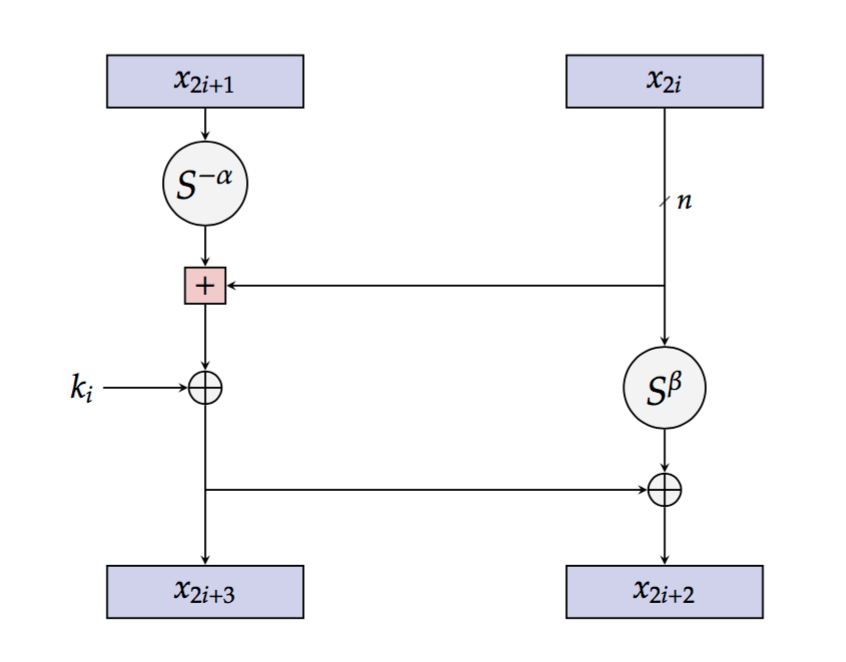
\includegraphics[width=0.4\textwidth]{speck.png}
\caption{The SPECK Round function}
\label{fig:speck}
\end{figure}


\section{Why embedded cryptography?}
Why is it useful to create cryptographic hardware instead of using software implementations? Firstly and most obviously, a dedicated hardware implementation achieves better performance. More importantly, a separate cryptography processor creates an explicit physical barrier around sensitive information. Cryptographic software performed in an environment with other applications running concurrently can leak information through for example timing variations or the cache. It is better for secret keys to be handled in their own environment with a private cache. Furthermore, many devices in the Internet of Things have limited resources or even no generalized core at all, in which case cryptography in hardware is the only option. 


\section{Practical}
Apart from implementing the SPECK encryption algorithm, we will have to provide our own compiler toolchain, tests and working infrastructure. We however do have a reference implementation available in the original paper \cite{speck} and a set of test vectors to check for correctness. 


\footnotesize
\bibliographystyle{plain}
\bibliography{refs}


 
\end{document}